\documentclass[aps,reprint]{revtex4-1}
% Engine-specific settings
% Detect pdftex/xetex/luatex, and load appropriate font packages.
% This is inspired by the approach in the iftex package.
% pdftex:
\ifx\pdfmatch\undefined
\else
    \usepackage[T1]{fontenc}
    \usepackage[utf8]{inputenc}
\fi
% xetex:
\ifx\XeTeXinterchartoks\undefined
\else
    \usepackage{fontspec}
    \defaultfontfeatures{Ligatures=TeX}
\fi
% luatex:
\ifx\directlua\undefined
\else
    \usepackage{fontspec}
\fi
% End engine-specific settings
\usepackage[english]{babel}
\usepackage{csquotes}
% \usepackage[backend=biber, sortcites]{biblatex}
\usepackage{url}
\usepackage{textcomp}
\usepackage[usenames,dvipsnames,svgnames, table]{xcolor}
\usepackage[font={scriptsize}]{caption}
\usepackage{amsmath} \usepackage{amsthm} \usepackage{amsfonts}
\usepackage{amssymb}
\usepackage{enumerate}
\usepackage{tikz} \usepackage{float}
\usetikzlibrary{patterns}
\usepackage[procnames]{listings}
\usepackage{pstool} \usepackage{pgfplots}
\usepackage{wrapfig} \usepackage{graphicx} \usepackage{epstopdf}
\usepackage{afterpage}
\usepackage{physics}
\usepackage{multirow}
\usepackage{gensymb}
\usepackage{algorithm}
\usepackage{microtype}
\usepackage[noend]{algpseudocode}
\usepackage{xcolor,colortbl}
\usepackage{microtype}
\usepackage{geometry}
\usepackage{hyperref}
\usepackage{graphicx}
\usepackage{caption}
\usepackage{subcaption}
\usepackage{lipsum}
% \usepackage{pythontex}
% \usepackage{authblk}
\usepackage{nth}
\usepackage{siunitx}
% \usepackage[toc,page]{appendix}
\floatstyle{plaintop}
\restylefloat{table}

% Custom commands
\newcommand{\unit}[1]{\:\mathrm{#1}}
\newcommand{\noref}[1]{\hyperref[#1]{\ref*{#1}}}
\newcommand{\nonref}[1]{\hyperref[]{\ref*{#1}}}
\newcommand\blankpage{%
  \null
  \thispagestyle{empty}%
  \addtocounter{page}{-1}%
  \newpage}

% Default fixed font does not support bold face
\DeclareFixedFont{\ttb}{T1}{txtt}{bx}{n}{7} % for bold
\DeclareFixedFont{\ttm}{T1}{txtt}{m}{n}{7}  % for normal

\newcommand\numberthis{\addtocounter{equation}{1}\tag{\theequation}}
\DeclareCaptionFont{white}{\color{white}}
\DeclareCaptionFormat{listing}{\colorbox{gray}{\parbox{\columnwidth}{#1#2#3}}}
\pgfplotsset{compat=1.14} %TODO: Setting this removed several error messages, should it be here!?
\def\axislength{.5}

% Colors
\colorlet{MyColorOne}{blue!35}
\newcommand{\lightercolor}[3]{% Reference Color, Percentage, New Color Name
    \colorlet{#3}{#1!#2!white}
}
\newcommand{\darkercolor}[3]{% Reference Color, Percentage, New Color Name
    \colorlet{#3}{#1!#2!black}
}
\lightercolor{MyColorOne}{50}{MyColorOneLight}
\darkercolor{MyColorOne}{50}{MyColorOneDark}

\newcommand{\bigO}[1]{\ensuremath{\mathop{}\mathopen{}\mathcal{O}\mathopen{}\left(#1\right)}}

% Biber for references
% \bibliographystyle{aipauth4-1}

\begin{document}
\sisetup{detect-all}
\title{Finite element solutions to the diffusion equation in one and two dimensions}
\author{Erlend Lima}
\author{Frederik J. Mellbye}
\affiliation{University of Oslo, Oslo, Norway \\ Source code available at: \url{https://github.com/Caronthir/FYS3150/tree/master/Project3}}
\date{\today}

\begin{abstract}
Three finite element methods, namely the explicit forward Euler, implicit backward Euler
and Crank-Nicolson schemes are used to solve the diffusion equation in one and
two dimensions. The equation is derived and motivated for a Couette flow from the
incompressible Navier-Stokes equations, and a wide array of other applications
are discussed. The solutions are compared to known analytic solutions, which shows
that the second order in time and space Crank-Nicolson scheme consistently outperforms
the Euler methods in terms of solution accuracy. \textbf{TALL HER!} The stability limitations of the
explicit position-centered, time-forward Euler scheme are investigated and found to
correspond to the expected requirement $\Delta{t}/\Delta{x}^2 \leq 1/2$ in one dimension.
\end{abstract}
\maketitle
\tableofcontents
\makeatletter
\let\toc@pre\relax
\let\toc@post\relax
\makeatother

\newpage

\section{Introduction} \label{sec:introduction}
The diffusion equation is a partial differential equation that appears frequently in
multiple fields of science. Among others, heat transfer processes, Markov processes
and applications in life science are examples of situations where the equation describes
some phenomena. Furthermore, the numerical methods that are used to solve the diffusion
equation are easily modified to solve similar equations, which demonstrates the relevance
of investigating the methods and attributed stability conditions and errors.

In this paper the diffusion equation is derived for a one-dimensional shear-stress
driven Couette flow from the incompressible Navier-Stokes equations. The resulting
equation along with the boundary and initial conditions are scaled and discretized.
Three numerical methods are employed to solve the equation, namely the explicit Forward and
implicit Backward Euler methods, and a combination of the two, the Crank-Nicolson scheme.
The solutions from the numerical methods are compared to the analytical solution, which
shows a close agreement. The solver is then extended to solve the two dimensional
diffusion equation, which for instance can be used to describe heat flow in a
plate with edges held at given temperatures.
\section{Theory} \label{sec:theory}
\subsection{Deriving the diffusion equation for a Couette flow}
A Couette flow is a drag-induced flow between either parallel plates or concentric
rotating cylinders and therefore differs from pressure driven flows such as the
Hagen-Poiseuille flow. It is assumed that the flow is laminar and of an incompressible
Newtonian fluid of density $\rho$ and vicosity $\mu$ between infinite parallel
plates located at $y = 0$ and $y = L$. The situation is illustrated in figure~\ref{fig:couette}.
Initially, the plates and the fluid is at rest, but at some time $t = t_0$
the upper plate is given a horizontal velocity $U$.
\begin{figure}[H]
  \centering
  \begin{tikzpicture}
    % \draw[help lines, thick, dashed, opacity=0.5] (0,0) grid (8,4);
    \draw (0,0) -- (6,0) node[anchor=north] {$y = 0$};
    \draw (0,3) -- (6,3) node[anchor=south] {$y = L$};

    \draw[->, thick] (2,3.2) -- (4,3.2);
    \node at (3,3.4) {$U$};
    \node at (5,1.5) {$\rho, \mu$};

    \draw[MyColorOne,dashed] (4,3) -- (2,0);
    \draw[MyColorOne,dashed] (2,0) -- (2,3);
    \foreach \y in {0.5,1,...,2.5} {%
      \draw[->, MyColorOneDark, thick] (2,\y) -- (2 + 2*\y/3,\y);
    }%

    \coordinate (O) at (0,0.1);
    \coordinate (x) at (\axislength,0.1);
    \coordinate (y) at (0,\axislength+.1);
    \draw[->] (O) -- (x) node[above] {$x$};
    \draw[->] (O) -- (y) node[right] {$y$};

    \fill[pattern=north west lines] (0,-.1) rectangle ++(6,.1);
    \fill[pattern=north west lines] (0,3) rectangle ++(6,.1);
  \end{tikzpicture}
  \caption{Couette flow between two parallel plates. The horizontal distance
  scale is $\gg L$, so the plates are considered infinite in the $x$ and $z$
  directions. The flow is here at a fully developed stage.}
  \label{fig:couette}
\end{figure}
The Navier-Stokes equations govern the time development of the fluid velocity field.
The momentum equation reads
\begin{align*}
  \pdv{\vb{u}}{t} + (\vb{u} \cdot \nabla) \vb{u} = - \frac{1}{\rho} \nabla p + \nu \nabla^2 \vb{u}
\end{align*}
where $\nu = \mu/\rho$ is the kinematic viscosity, and the incompressibility
condition is
\begin{align*}
  \nabla \cdot \vb{u} = 0
\end{align*}
The only force acting on the system is the tangential shear stress in the
horizontal direction, and the velocity field is therefore assumed to be on the
form $\vb{u} = (u,v = 0,w = 0)$. The pressure gradient term is eliminated because the
pressure is constant, and the inertial term vanishes because of the incompressibility
condition. The equations reduce to
\begin{align}
  \pdv{u}{t} = \nu \pdv[2]{u}{y}
\end{align}
which is the diffusion equation. The no-slip boundary condition applies to both
surfaces, so
\begin{align*}
  u(y = L) &= U \\
  u(y = 0) &= 0
\end{align*}
To generalize the results the equations are scaled and written in terms of
a spatial variable $x$ instead of $y$:
\begin{align}
  \pdv{\hat{u}}{\hat{t}} = \pdv[2]{\hat{u}}{\hat{x}}
\end{align}
where $\hat{x} = x / L$ and $\hat{u} = u / U$ and thus $\hat{t} = t / (L^2 / \nu)$ are dimensionless quantities.
The initial conditions are converted to $\hat{u}(\hat{x},0) = 0$ for $0 < \hat{x} < 1$,
and $\hat{u}(0,\hat{t}) = 0$ and $\hat{u}(1,\hat{t}) = 1$ at the boundaries for $\hat{t} > 0$.
Only the dimensionless equation is considered hereafter, with the hats omitted.
\subsection{Developing the numerical algorithms}
In this project three numerical methods for solving partial differential equations (PDEs)
are used. The methods are the explicit forward and implicit backward Euler
algorithms, along with the implicit Crank-Nicolson scheme. For all three schemes
position, time and thus velocity is discretized:
\begin{align*}
  t &\rightarrow t_j = t_0 + j \Delta{t} \\
  x &\rightarrow x_i = x_0 + i \Delta{x} \\
  u(x,t) &\rightarrow u(x_i, t_i)
\end{align*}
where $0 < i < n + 1$ and $j \geq 0$. The position step size is given by $\Delta{x} = 1 /(n+1)$.
The notation $u(x_i,t_i) = u_{i,j}$ is used. The following derivations are based on
section 10.2 in \cite{mortenjensen}, which has more detailed explanations.
\subsubsection{Explicit forward Euler scheme}
Perhaps the simplest method for forwarding the positions as a function of time
is the forward Euler method. The derivatives are approximated using
\begin{align*}
  \pdv{u}{t} &= \frac{u_i,j+1 - u_i,j}{\Delta{t}} + \bigO{\Delta{t}} \\
  \pdv[2]{u}{x} &= \frac{u_{i+1,j} - 2 u_{i,j} + u_{i-1, j}}{\Delta{x}^2} + \bigO{\Delta{x}^2}
\end{align*}
Inserting these expressions in the diffusion equation, omitting the error terms
and setting $\alpha = \Delta{t} / \Delta{x}^2$ yields the explicit scheme
\begin{align} \label{eq:explicitscheme}
  u_{i,j+1} = \alpha u_{i_1,j} + (1-2\alpha) u_{i,j} + \alpha u_{i+1,j}
\end{align}
Given initial and boundary values, the succeding steps can be calculated using~\ref{eq:explicitscheme},
all the terms on the right hand side are known and therefore explicitly give
the solution in the next step. The above equation can be rewritten to a matrix-vector
multiplication
\begin{align*}
  \vb{u}_{j+1} = A \vb{u}_j
\end{align*}
where the entries in $\vb{u}_j$ are the $u_i$'s at time $t_j$ and the matrix $A$ is
given by
\begin{align*}
  A = \begin{bmatrix}
        1 - 2\alpha & \alpha      & 0            & \hdots  & 0      \\
        \alpha      & 1 - 2\alpha & \alpha       & 0       & \vdots \\
        0           & \alpha      & 1 - 2\alpha  & \alpha  & \vdots \\
        \vdots      & \ddots      & \ddots       & \ddots  & \vdots \\
        0           & \hdots      & \hdots       & \alpha  & 1 - 2\alpha \\
      \end{bmatrix}
\end{align*}
The discretized PDE can therefore be written as a chain of matrix multiplications
\begin{align*}
  \vb{u}_{j} = A^{j} \vb{u}_0
\end{align*}
where $\vb{u}_0 = g(x)$ is the initial state.
\subsubsection{Implicit backward Euler}
For the implicit backward Euler method the derivation is almost identical,
the difference originates at the backward Euler time derivative expansion
\begin{align*}
  \pdv{u}{t} = \frac{u_{i,j} - u_{i,j-1}}{\Delta{t}} + \bigO{\Delta{t}}
\end{align*}
which yields the implicit steps
\begin{align*}
  u_{i,j-1} = -\alpha u_{i_1,j} + (1-2\alpha) u_{i,j} - \alpha u_{i+1,j}
\end{align*}
Note that $\alpha$ is the same as in the forward Euler scheme. As in the previous
scheme, a time step is solved through a matrix equation
\begin{align*}
  A \vb{u}_{j} = \vb{u}_{j-1}
\end{align*}
where
\begin{align*}
  A = \begin{bmatrix}
        1 + 2\alpha & -\alpha      & 0            & \hdots  & 0      \\
        -\alpha      & 1 + 2\alpha & -\alpha       & 0       & \vdots \\
        0           & -\alpha      & 1 + 2\alpha  & -\alpha  & \vdots \\
        \vdots      & \ddots      & \ddots       & \ddots  & \vdots \\
        0           & \hdots      & \hdots       & -\alpha  & 1 + 2\alpha \\
      \end{bmatrix}
\end{align*}
Each step is a backwards step, however if the matrix is constant in time it only
needs to be inverted once. The solution at time $t_j$ is therefore given by
\begin{align*}
  \vb{u}_j = A^{-j} \vb{u}_0
\end{align*}
\subsubsection{Crank-Nicolson scheme}
The Crank-Nicolson scheme combines the ideas from the above Euler methods and is
a second-order implicit method in time. Using the Taylor expansions seen in
\cite{mortenjensen}, the diffusion equation can be rewritten to
\begin{align*}
  -\alpha u_{i_1, j} &+ (2 + 2\alpha) u_{i,j} - \alpha u_{i+1,j}\\
   &= \alpha u_{i-1,j-1} + (2 - 2\alpha) u_{i, j-1} + \alpha u_{i+1,j-1}
\end{align*}
where $\alpha$ is the same as in the other methods. In matrix-vector form this
is equivalent to
\begin{align*}
  (2 I + \alpha B) \vb{u}_j = (2 I - \alpha B) \vb{u}_{j-1}
\end{align*}
where the solution vectors $\vb{u}$ are the same as before, $I$ is the identity
matrix and $B$ is given by
\begin{align*}
  B = \begin{bmatrix}
        2  & -1 & \hdots  & 0      \\
        -1 & 2  & -1 & 0       & \vdots \\
        0  & -1 & 2  & -1  & \vdots \\
        \vdots       & \ddots      & \ddots       & \ddots  & \vdots \\
        0  & \hdots  & \hdots       & -1  & 2 \\
      \end{bmatrix}
\end{align*}
Rewriting the above equation, the Crank-Nicolson scheme is
\begin{align*}
  \vb{u}_j = (2 I + \alpha B)^{-1} (2 I - \alpha B) \vb{u}_{j-1}
\end{align*}
\subsection{Algorithm stability and trunctation errors}
The algorithms have different accuracies and are limited by different stability
conditions. The solution approaches definite values if the spectral radius $\rho(A)$ of
the matrix $A$ satisfies
\begin{align} \label{eq:spectralradius}
  \rho(A) = \text{max}\{ |\lambda| : \text{det}(A - \lambda I) = 0 \} < 1
\end{align}
i.e. the maximum absolute eigenvalue can not exceed unity. From this is follows
that positive definite matrices always satisfy~\ref{eq:spectralradius}.

In addition to the stability requirement there will obviously be trunctation errors
for each scheme. The requirements are summarized in table~\ref{table:errors} and derived in the
appendix, see~\ref{sec:errors}.
\begin{table}[H]
\centering
\caption{Summarized trunctation errors and stability requirements for the schemes.}
\label{table:errors}
\begin{tabular}{p{0.31\linewidth}|p{0.34\linewidth}|p{0.28\linewidth}}
\hline
Scheme         & Trunctation Error                          & Stability requirement                     \\ \hline
Crank-Nicolson & $\bigO{\Delta{x^2}}$, $\bigO{\Delta{t^2}}$ & None                                      \\
Forward Euler  & $\bigO{\Delta{x^2}}$, $\bigO{\Delta{t}}$   & $\Delta{t} \leq \frac{1}{2} \Delta{x^2}$  \\
Backward Euler & $\bigO{\Delta{x^2}}$, $\bigO{\Delta{t}}$   & None                                      \\ \hline
\end{tabular}
\end{table}
\subsection{Analytic solution for the 1-D diffusion equation} \label{sec:analytic1d}
Analytic solutions are available for the one-dimensional diffusion equation. Assume
the differential equation is scaled and on the form
\begin{align*}
  \pdv[2]{u}{x} = \pdv{u}{t}
\end{align*}
with initial conditions
\begin{align*}
  u(x,0) = g(x) \qquad 0 < x < L
\end{align*}
and constant boundary conditions
\begin{align*}
  u(0,t) = 0 \qquad u(L,t) = 1 \qquad t \geq 0
\end{align*}
Using separation of variables, the solution is assumed to be on the form
$u(x,t) = X(x)T(t)$. Inserting this in the diffusion equation yields
\begin{align*}
  \frac{1}{X} \pdv[2]{X}{x} = \frac{1}{T} \pdv{T}{t}
\end{align*}
The left hand side of the equation is only a function of $x$, and the right hand
side similarly depends only on $t$. Thus both sides must be constant (set to $-\lambda^2$).
The PDE is therefore transformed to two ODE's:
\begin{align*}
  \pdv[2]{X}{x} + \lambda^2 X &= 0 \\
  \pdv{T}{t}    + \lambda^2 T &= 0
\end{align*}
which have general solutions
\begin{align*}
  X(x) &= A\sin{(\lambda x)} + B\cos{(\lambda x)} \\
  T(t) &= Ce^{-\lambda^2 t}
\end{align*}
The boundary conditions demand $B = 0$ and $\lambda = n \pi /L$ for $n = 1,2,\hdots$.
This yields solutions
\begin{align*}
  u(x,t) = A_n \sin{(n\pi x/L)}e^{-n^2 \pi^2 t/ L^2}
\end{align*}
Linear combinations of these solutions are also solutions because the diffusion
equation is linear. Thus
\begin{align}
  u(x,t) = \sum_{n = 1}^{\infty} A_n \sin{(n\pi x/L)}e^{-n^2 \pi^2 t/ L^2}
\end{align}
is a solution to the equation. The Fourier coefficients $A_n$ are determined
from the initial condition $u(x,0) = g(x)$. This is done by mapping the initial
configuration to the Fourier series base, through the inner product
\begin{align*}
  A_n = \frac{2}{L}\int_0^L g(x) \sin{(n \pi x / L)} \dd{x}
\end{align*}
\subsection{Two dimensions}
In two spatial dimensions, the diffusion equation is extended to
\begin{align} \label{eq:diffusion2d}
  \nabla^2 u = \pdv[2]{u}{x} + \pdv[2]{u}{y} = \pdv{u}{t}
\end{align}
where the solution $u(x,y,t)$ is a function of time $t$ and two spatial coordinates $x$ and $y$,
the problem is therefore $2 + 1$ dimensional. $\nabla^2$ is the Laplacian. The solution at
each time step is now a two-dimensional grid, which needs to be enclosed by boundary
conditions in two dimensions.
\subsubsection{Explicit scheme}
The simplest method for approximating a solution to the two-dimensional diffusion
equation is an explicit forward scheme. The derivatives are approximated as above:
\begin{align*}
  \pdv[2]{u}{x} &= \frac{u^l_{i+1,j} - 2u^l_{i,j} + 2u^l_{i-1,j}}{h^2} \\
  \pdv[2]{u}{y} &= \frac{u^l_{i,j+1} - 2u^l_{i,j} + 2u^l_{i,j-1}}{h^2} \\
  \pdv{u}{t} &= \frac{u^l_{i,j} - u^{l-1}_{i,j}}{\Delta{t}}
\end{align*}
where $i$ and $j$ are node indices in space and $l$ represents the time steps. It
is here assumed that the lattice is a square so $h = \Delta{x} = \Delta{y}$. Inserting
these expressions in~\ref{eq:diffusion2d} yields
\begin{align*}
  u_{i,j}^{l+1} = u_{i,j}^l + \alpha (u^l_{i+1,j} + u^l_{i-1,j} + u_{i,j+1}^l + u_{i,j-1}^l - 4 u^l_{i,j})
\end{align*}
where $\alpha = \Delta{t}/h^2$. The right hand side is only a function of known
quantities (current state and boundary conditions), and therefore explcitly gives
the solution in the next step.
\subsection{Analytic solution to the two-dimensional diffusion equation}
There is also a closed form solution available for the two-dimensional diffusion equation.
Assume there are some boundary conditions (set to Dirichlet conditions here):
\begin{align*}
  u(0, y, t) = u(L, y, t) = u(x, 0, t) = u(x, L, t) = 0
\end{align*}
where the lattice length is $L$. These expressions simply state that the solution
value is held to $0$ at the edges, for instance fixed at some temperature or fluid
boundary flow velocity. The initial condition is some initial configuration given by a function $u(x,y,0) = g(x,y)$.
The same method is used here as in the one-dimensional case: separation of variables. The solution
is written as $u(x,y,t) = X(x) Y(y) T(t)$, and inserted in the heat equation. Each resulting
term must equal a constant $-\lambda^2$:
\begin{align*}
  X'' + \lambda^2 X &= 0 \\
  Y'' + \lambda^2 Y &= 0 \\
  T'  + \lambda^2 T &= 0
\end{align*}
where $X(0) = Y(0) = X(L) = Y(L) = 0$. From~\ref{sec:analytic1d} the solutions are
\begin{align*}
  X = A \sin{(\lambda x)} \quad Y = B \sin{(\lambda y)} \quad T = e^{-\lambda^2 t}
\end{align*}
Where the cosine terms vanish because of the boundary conditions. The upper
boundary conditions again yield $\lambda = n \pi / L$. Linear combinations
are solutions, so
\begin{align*}
  &u(x,y,t) = \\&\sum_{n = 1}^{\infty} A_{n} \sin{(n \pi x / L)} \sin{(n \pi y / L)} e^{- t n^2 \pi^2 / L^2}
\end{align*}
is a general solution, where again the coefficients need to be determined based
on the initial state.
\section{Method} \label{sec:method}
The full implementation of the algorithms is available in the Git-repository.
The one dimensional solver was implemented in C++, and to test the speed of
a vectorized NumPy implementation the two-dimensional solver was implemented in Python.
\subsection{Initial and boundary values. Implementations.}
\subsubsection{Testing the numerical solver}
To test the numerical solvers a specific case with a trivial analytic solution
was investigated. With an initial state of a half sine wave spanning the domain
\begin{align*}
  g(x) = \sin{(x \pi)}
\end{align*}
and Dirichlet boundaries $u(0,t) = u(1,t) = 0$ an analytic solution can be found.
Observe that the general solution terms are very similar to the initial condition,
because setting $t = 0$ removes the exponential factor. Furthermore, using only
the $n = 1$ term yields $u(x,0) = g(x)$, and the solution in the test case is
\begin{align*}
  u(x,t) = \sin{(\pi x)} e^{- \pi^2 t}
\end{align*}
This solution is then tested against the numerical solutions for different step
sizes, both in space and time.
\subsubsection{Couette flow initial and boundary conditions}
For the Couette flow investigated in this paper, the zero flow initial condition
is $u(x,0) = 0$ for $0 < x < 1$. With a scaled plate velocity difference, the
lower plate at $x = 0$ is held stationary and the upper plate is given a constant
velocity $1$. This equates to boundary conditions $u(0,t) = 0$ and $u(1,t) = 1$.
\subsubsection{Two-dimensional boundaries}
In two dimensions, boundary conditions along all sides of the square lattice need
to be specified in addition to an initial state. The boundaries will be different
in differend cases, for instance one edge of a metal plate may be held at a much
higher temperature than the other sides. In the analysis in this paper, the boundaries
are set to Dirichlet boundaries, i.e.
\begin{align*}
  u(0,y,t) = u(1,y,t) = u(x,0,t) = u(x,1,t) = 0
\end{align*}
so all the edges have the same temperature. The grid could in this case also represent an
intersection of a square tube with flowing fluid and the tube stationary. With no
pressure driving the flow, the velocity field will diffuse away as energy is dissipated
to other forms through viscous effects.

For this paper only the explicit method is used to solve the two-dimensional equation.
The stability condition is tested by attempting to run the solver for combinations
of $\Delta t$ og $\Delta x$
\subsection{Matrix equation solver}
To solve the matrix equations some numerical method needs to be used. By inspection,
the matrices in all of the methods are tridiagonal, which allows usage of the
Thomas algorithm, specifically made to solve tridiagonal matrix systems. A
thorough derivation and analysis of the algorithm is seen in~\cite{project1}. The
implementation of the full solver can be seen in the source code.
\subsection{Error analysis}
Assume the solution at time step $j$ and node $i$ is $u_{i,j}$, and that the analytical
solution at the same position and time is $v_{i,j}$. The maximum relative error for some
time step is here defined as
\begin{align*}
  \epsilon_j \equiv \text{max }\left| \frac{u_{i,j} - v_{i,j}}{v_{i,j}}\right|
\end{align*}
where $i$ runs through discretized domain. This quantity is calculated for each
time step to show how the errors develop with time for each method, which is
then compared with the expected error orders in time for each scheme.
\section{Results} \label{sec:results}
\subsection{One dimensional solution}
There are two sets of results for the one dimensional case, first the sinusoidal
test case solution is presented, then the Couette flow results are shown.
\subsubsection{Half wave solution and errors}
See figures~\ref{fig:sinnumanalytic} through~\ref{fig:sinrelerr} for the solution
time development and the error as a function of time.
\begin{figure}[ht]
  \centering
  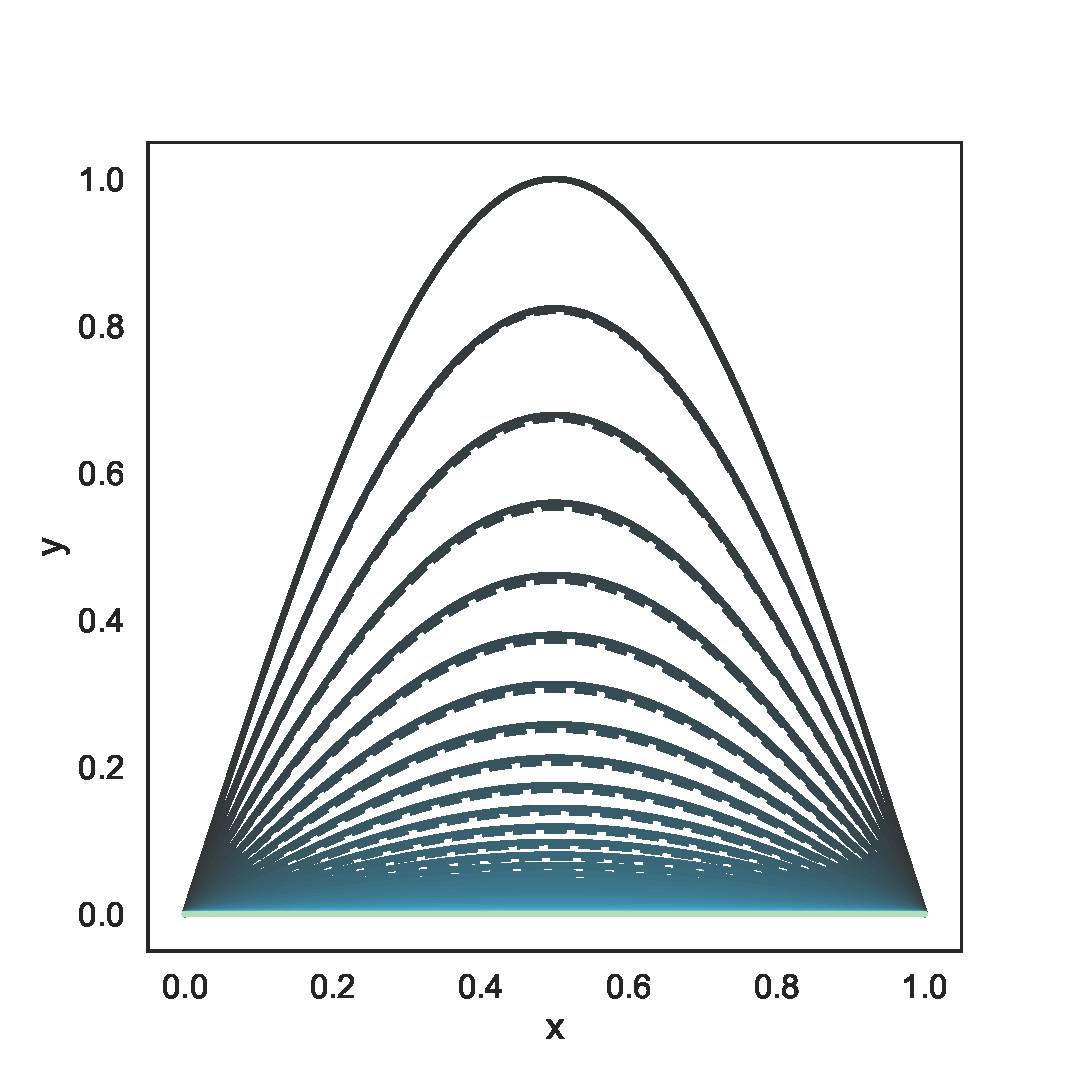
\includegraphics[width=\columnwidth]{figures/sin_numeric_vs_analytical.eps}
  \caption{\label{fig:sinnumanalytic} Both the numerical (solid) and analytical
    (dashed) solutions of the test case with
    sinusoidal initial conditions. Brighter colors represent later time points.}
\end{figure}
\begin{figure}[ht]
  \centering
  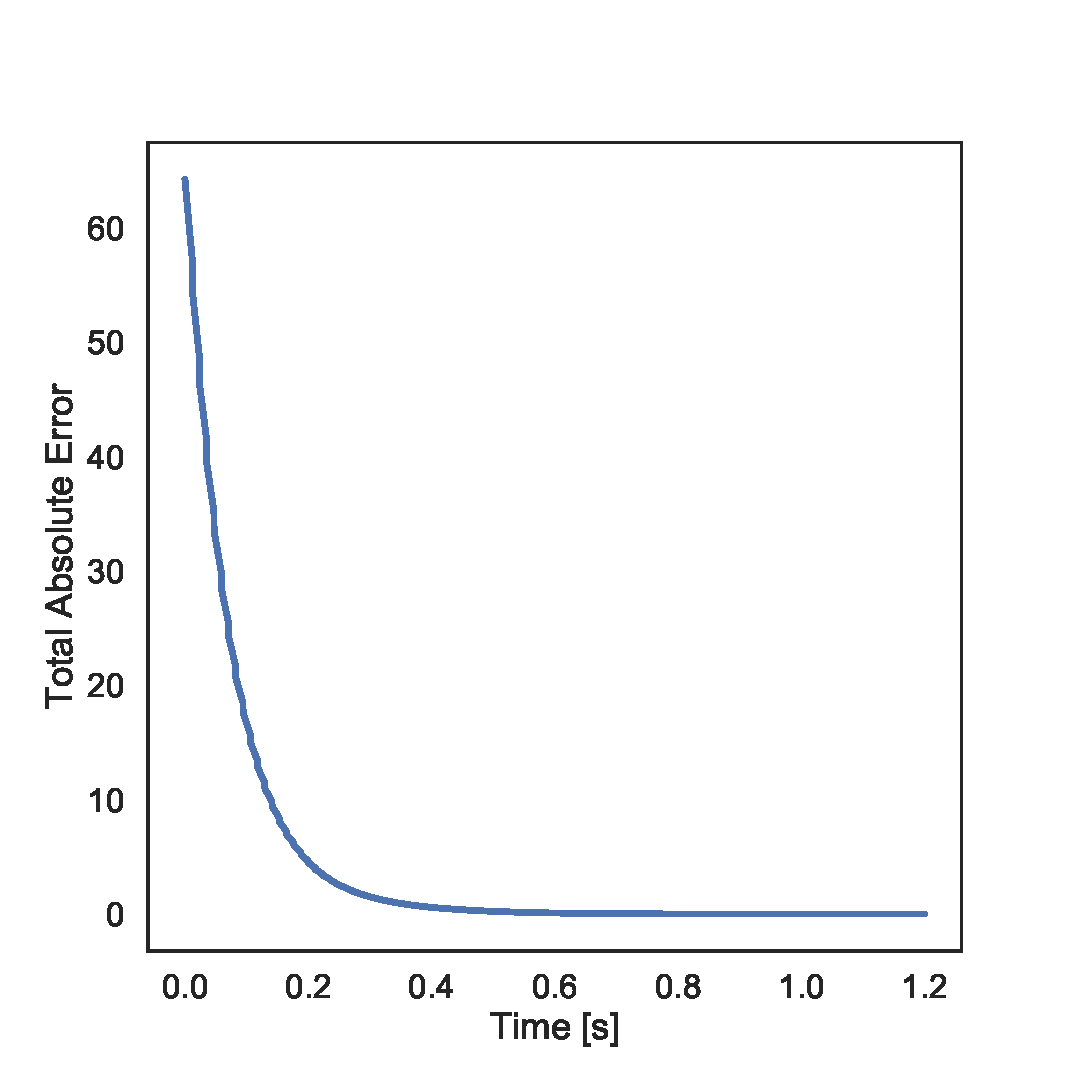
\includegraphics[width=\columnwidth]{figures/sin_absolute_error.eps}
  \caption{\label{fig:sinabserr} The total absolute error in the test case.}
\end{figure}
\begin{figure}[ht]
  \centering
  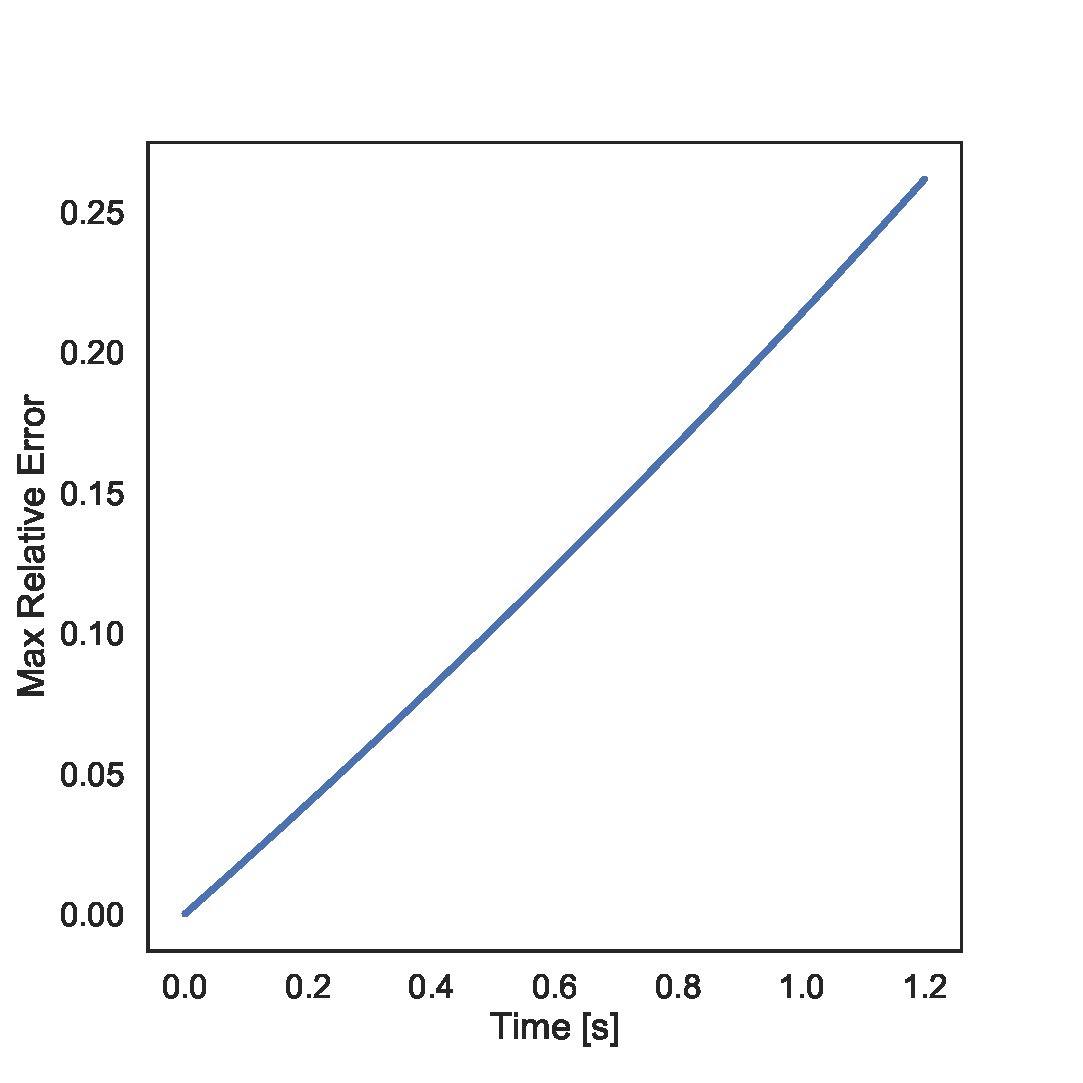
\includegraphics[width=\columnwidth]{figures/sin_relative_error.eps}
  \caption{\label{fig:sinrelerr} The total relative error in the test case.}
\end{figure}
\subsubsection{Couette flow solution}
The time development with the explicit scheme for the Couette flow is shown in
figure~\ref{fig:couettenumanalytic}, with the analytic solution.
\begin{figure}[ht]
  \centering
  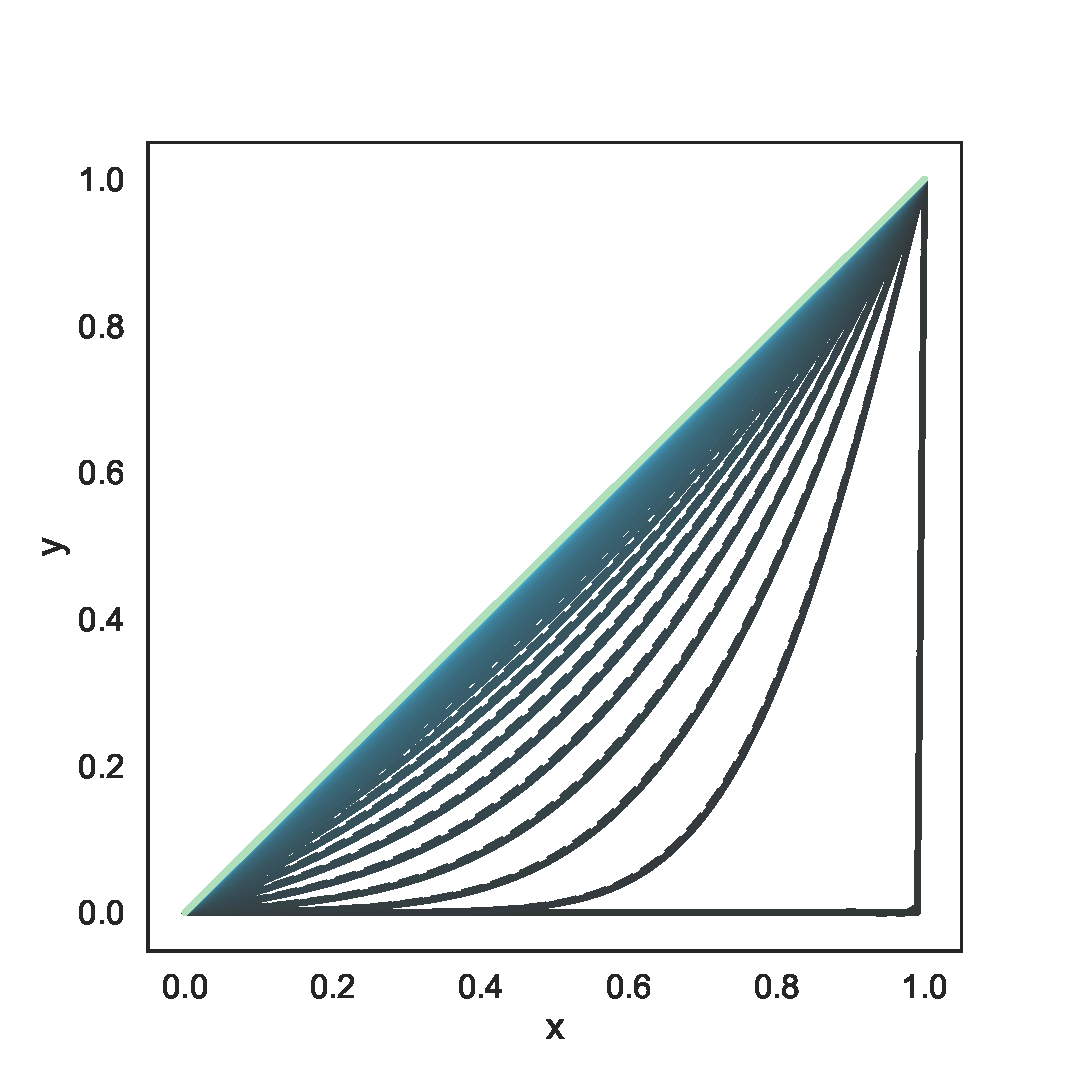
\includegraphics[width=\columnwidth]{figures/couette_numeric_vs_analytical.eps}
  \caption{\label{fig:couettenumanalytic} Both the numerical (solid) and analytical
    (dashed) solutions of the Couette flows. Brighter colors represent later time
    points.}
\end{figure}
Then compare with analytic result.
\subsection{Two dimensional solution}
The two-dimensional solution time development is shown in figure~\ref{fig:twodimsolution}.
The initial configuration is $u(x,y,0) = \sin{(\pi x)} \sin{(\pi y)}$, where
$0 < x,y < 1$.
\begin{figure}[ht]
  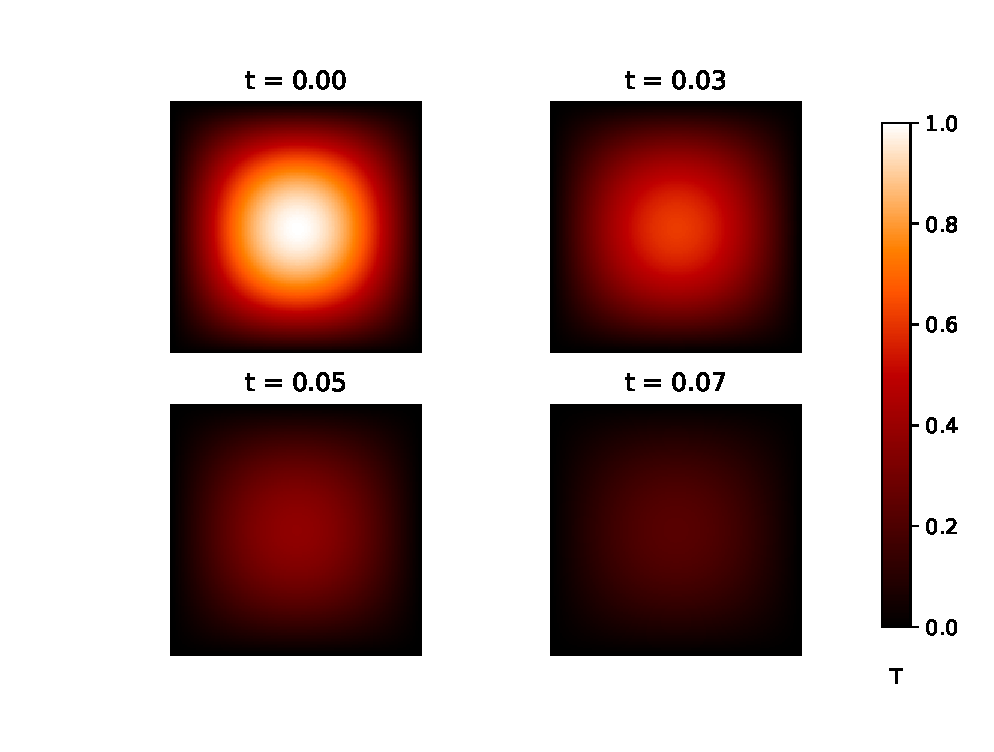
\includegraphics[width=\columnwidth]{figures/twodim.eps}
  \caption{Two dimensional solution for four different time steps with a
  $101 \times 101$ grid, $\Delta x = 10^{-2}$, $\Delta t = 2.5 \times 10^{-5}$
  and Dirichlet boundaries. This combination sets $\alpha = 0.25$, right on the stability limit.
  Also note that bicubic interpolation is used to produce smoother figures.
  }
  \label{fig:twodimsolution}
\end{figure}
Also, see figure~\ref{fig:twodimamplitude} for the center node (technically all four
center nodes) amplitude as a function of time.
\begin{figure}[ht]
  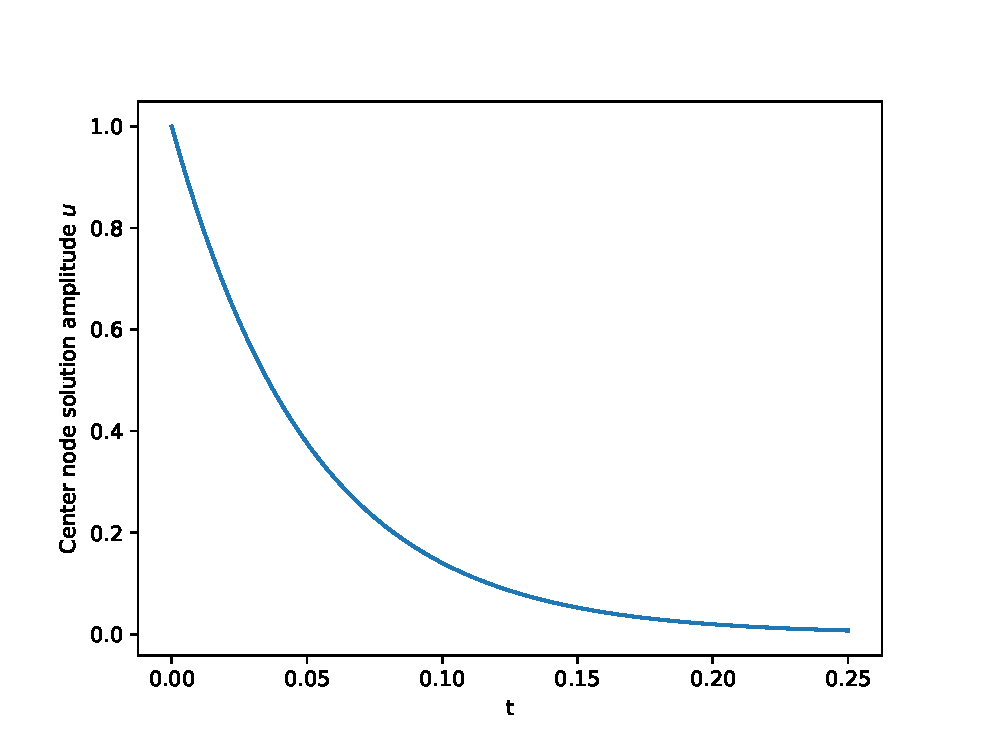
\includegraphics[width=\columnwidth]{figures/twodimamplitude.eps}
  \caption{Center node amplitude for the two dimensional solution, with a longer
  time period}
  \label{fig:twodimamplitude}
\end{figure}
\section{Discussion} \label{sec:discussion}
\subsection{One dimensional equation}
\subsubsection{Test case - Verifying the implementation}
By inspecting the solution when the initial configuration is half a sine wave
shown in figure~\ref{fig:sinnumanalytic}, it is clear that the numerical solution
behaves as expected and very similar to the analytic expression. The amplitude
declines in a similar manner to how heat would escape or how the fluid flow would
gradually be put to a halt in a tube in which the pressure difference was to be
switched off. Furthermore, the solution corresponds well with the analytic solution
despite the increasing deviation with time. The increasing error is also clear from
figure~\ref{fig:sinrelerr}. These results are for the explicit method.
\subsubsection{Couette flow solution}
The Couette flow solution shown in figure~\ref{fig:couettenumanalytic} also behaves
as expected. The upper boundary movement gradually accelerates more and more of the fluid through
viscosity, and the solution approaches the expected linear equilibrium flow state
with time. The Newtonian viscous forces transfer momentum across the fluid, which
is one of the key types of possible diffusion processes.
\subsection{Two dimensional equation}
The explicit method two dimensional solution inhibits very similar characteristics
as 
\section{Conclusion} \label{sec:conclusion}
\bibliography{references}
\blankpage
\appendix
\section{Derivation of trunctation errors and stability conditions} \label{sec:errors}
\subsection{Explicit scheme}
The explicit scheme uses standard approximations for the derivatives which are
inserted in the diffusion equation. The first order time approximation has
an error term $\sim \Delta{t}$, and the second derivative position approximation
has an error $\Delta{x^2}$. The method is therefore second order in position and
first order in time.

For the stability condition recall equation~\ref{eq:spectralradius}, which states
that the spectral radius $\rho$ of the matrix does not exceed $1$. If the scheme is
unstable, the algorithm will amplify trunctation and round-off errors, which is
now shown to be a possibility for the explicit scheme. The matrix
is rewritten to $A = I - \alpha B$, where
\begin{align*}
  B = \begin{bmatrix}
        2  & -1 & \hdots  & 0      \\
        -1 & 2  & -1 & 0       & \vdots \\
        0  & -1 & 2  & -1  & \vdots \\
        \vdots       & \ddots      & \ddots       & \ddots  & \vdots \\
        0  & \hdots  & \hdots       & -1  & 2 \\
      \end{bmatrix}
\end{align*}
$A$ therefore has eigenvalues $\lambda_i = 1 - \alpha \mu_i$ where $\mu_i$ is
the eigenvalues of $B$. The matrix elements of $B$ are $b_{i,j} = 2\delta_{i,j} - \delta_{i+1,j} - \delta{i-1,j}$.
For component $i$ the eigenequations are
\begin{align*}
  (B\vb{x})_i &= \sum_{j=1}^{n} (2\delta_{i,j} - \delta_{i+1,j} - \delta{i-1,j})x_j \\
              &= 2x_i - x_{i+1} - x_{i-1} \\
              &= \mu_i x_i
\end{align*}
Expanding $x$ in a basis of sines with arguments $\theta = l \pi / n + 1$, the previous equation can be rewritten as
\begin{align*}
  2(1 - \cos{(\theta)}) = \mu_i
\end{align*}
from which it is clear that the eigenvalues are $\mu_i = 2 - 2 \cos{(\theta)}$. The
spectral radius requirement is therefore
\begin{align*}
  -1 < 1 - 2 \alpha (1 - \cos{(\theta)}) < 1
\end{align*}
which is satisfied if $\alpha \leq 1/2$. Thus the stability requirement is
\begin{align}
  \frac{\Delta{t}}{\Delta{x^2}} \leq \frac{1}{2}
\end{align}
The explicit scheme for solving the one-dimensional diffusion equation is therefore
conditionally stable.

\subsection{Implicit scheme}
The implicit scheme uses the same time and position approximations as the explicit
scheme, and therefore has identical trunctation error orders. However, the matrix
is here positive definite, and the eigenvalues automatically satisfy~\ref{eq:spectralradius}.
The implicit scheme is therefore unconditionally stable.

\subsection{Crank-Nicolson scheme}
The derivation of the Crank-Nicolson scheme is similar to the above derivations,
but notice that the time derivative approximations are now of second order. The
matrix used in the algorithm is, as for the implicit Euler method, positive definite
and the Crank-Nicolson scheme is therefore also unconditionally stable.
\blankpage
\end{document}

% Local Variables:
% TeX-engine: luatex
% End:
